\lecture{个人简介}{lec:introduction}
\section[课程概况]{课程概况及要求}\label{sec:chap00-sec02}
%%%%%%%%%%%%%%%%%%%%%%%%%%%%%% 课程概况 %%%%%%%%%%%%%%%%%%%%%%%%%%%%%%%%%%%
\begin{frame}{课程概况}{预修课程和教材}
  \stretchon
  \begin{itemize}
  \item\hilite<1> {\bfseries 预修课程:}
    \begin{itemize}
    \item C语言程序设计(无法回避的\alert{指针})
    \item 高等数学(永远的\alert{根})
    \item 英语(要求不高,但你得\alert{不断用})
    \end{itemize}\pause         
  \item\hilite<2> {\bfseries 教材:}
    \begin{itemize}
    \item C++面向对象程序设计(第2版). 龚晓庆, 付丽娜, 朱新懿, 李康著. 北京:清华大学
      出版社. 2011.
    \end{itemize}
    \centering
    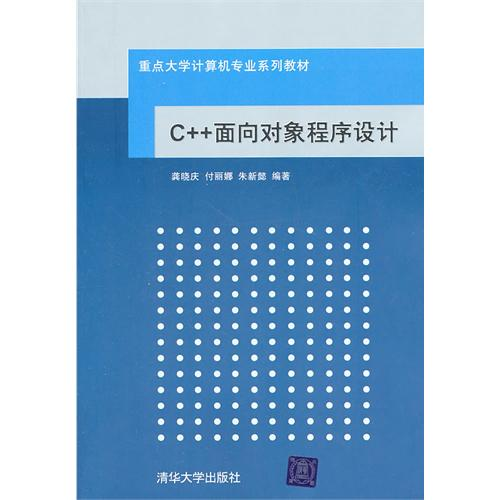
\includegraphics[height=0.4\textheight]{chap00/01textbook.jpg} %
  \end{itemize}
  \stretchoff
\end{frame}

\begin{frame}{课程概况}{参考资料}
  \stretchon
  \begin{itemize}
  \item\hilite<1> {\bfseries 参考资料:}    
    \begin{itemize}
    \item The C++ Programming Language, 4th Edition. Stroustrup,
      Bjarne. Addison-Wesley. 2013.
    \item C++ How to Program, 10th Edition. Paul Deitel, Harvey
      Deitel. Prentice Hall. 2016.
    \item Programming Abstractions in C++. Eric Roberts. Prentice Hall. 2013.
    \end{itemize}
    \centering
    
\includegraphics[height=0.35\textheight]{chap00/03programming.jpg} %
    \quad 
\includegraphics[height=0.35\textheight]{chap00/CHTP.jpg} %
    \quad 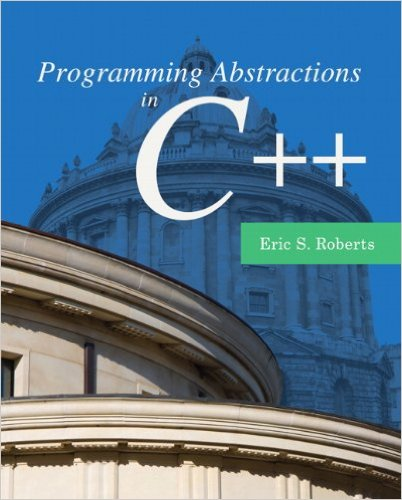
\includegraphics[height=0.35\textheight]{chap00/PAinCPP.jpg} %
  \end{itemize}
  \stretchoff
\end{frame}

\section[要求]{基本要求}\label{sec:chap00-sec03}
\begin{frame}{课程要求}{基本要求}
  \stretchon
  \begin{itemize}
  \item {\bfseries 考勤}(\alert{扣分制度})
    \begin{itemize}
    \item 课堂随机考勤
    \item 实习课随机考勤
    \end{itemize}
  \item  {\bfseries 成绩评定}
    \begin{itemize}
    \item 结业(期末)考试---\alert{70\%}
      \begin{itemize}
      \item 笔试(\alert{闭卷},拟定于XX周)
      \end{itemize}
    \item 平时成绩---\alert{30\%}
      \begin{itemize}
      \item 考勤      
      \item 在线评阅系统成绩(\url{http://202.117.179.201/contest.php?cid=1047})
      \item 大作业(论文分析或采用面向对象方法开发一个实用小软件)
      \end{itemize}
    \end{itemize}
  \end{itemize}
  \stretchoff
\end{frame}

\section[内容]{讲授内容}\label{sec:chap00-sec04}
\begin{frame}{课程内容}{讲授内容}
  \stretchon
  %\renewcommand{\labelenumi}{[\arabic{enumi}]} %
  % \begin{enumerate}
  % \item 第~\chinese{enumi}~章~面向对象基础%
  % \item 第~\chinese{enumi}~章~C++语言概览%
  % \item 第~\chinese{enumi}~章~C++语言基础%    
  % \item 第~\chinese{enumi}~章~复合类型
  % \item 第~\chinese{enumi}~章~函数%
  % \item 第~\chinese{enumi}~章~类和对象%
  % \item 第~\chinese{enumi}~章~对象的初始化、复制和销毁
  % \item 第~\chinese{enumi}~章~运算符重载%
  % \item 第~\chinese{enumi}~章~组合与继承%
  % \item 第~\chinese{enumi}~章~虚函数与多态性%
  % \item 第~\chinese{enumi}~章~模板与泛型编程%
  % \item 第~\chinese{enumi}~章~标准库容器和算法%
  % \item 第~\chinese{enumi}~章~异常处理
  % \end{enumerate}
  % %\renewcommand{\labelenumi}{[\arabic{enumi}]} %
  \begin{enumerate}
  \item 第~1~章~面向对象基础%
  \item 第~2~章~C++语言概览%
  \item 第~3~章~C++语言基础%    
  \item 第~4~章~复合类型
  \item 第~5~章~函数%
  \item 第~6~章~类和对象%
  \item 第~7~章~对象的初始化、复制和销毁
  \item 第~8~章~运算符重载%
  \item 第~9~章~组合与继承%
  \item 第~10~章~虚函数与多态性%
  \item 第~11~章~模板与泛型编程%
  \item 第~12~章~标准库容器和算法%
  \item 第~13~章~异常处理
  \end{enumerate}
  \stretchoff
\end{frame}

\begin{frame}{课程内容}{知识体系}
  \stretchon
  \begin{itemize}
  \item 思维导图
  \end{itemize}
  \centering
    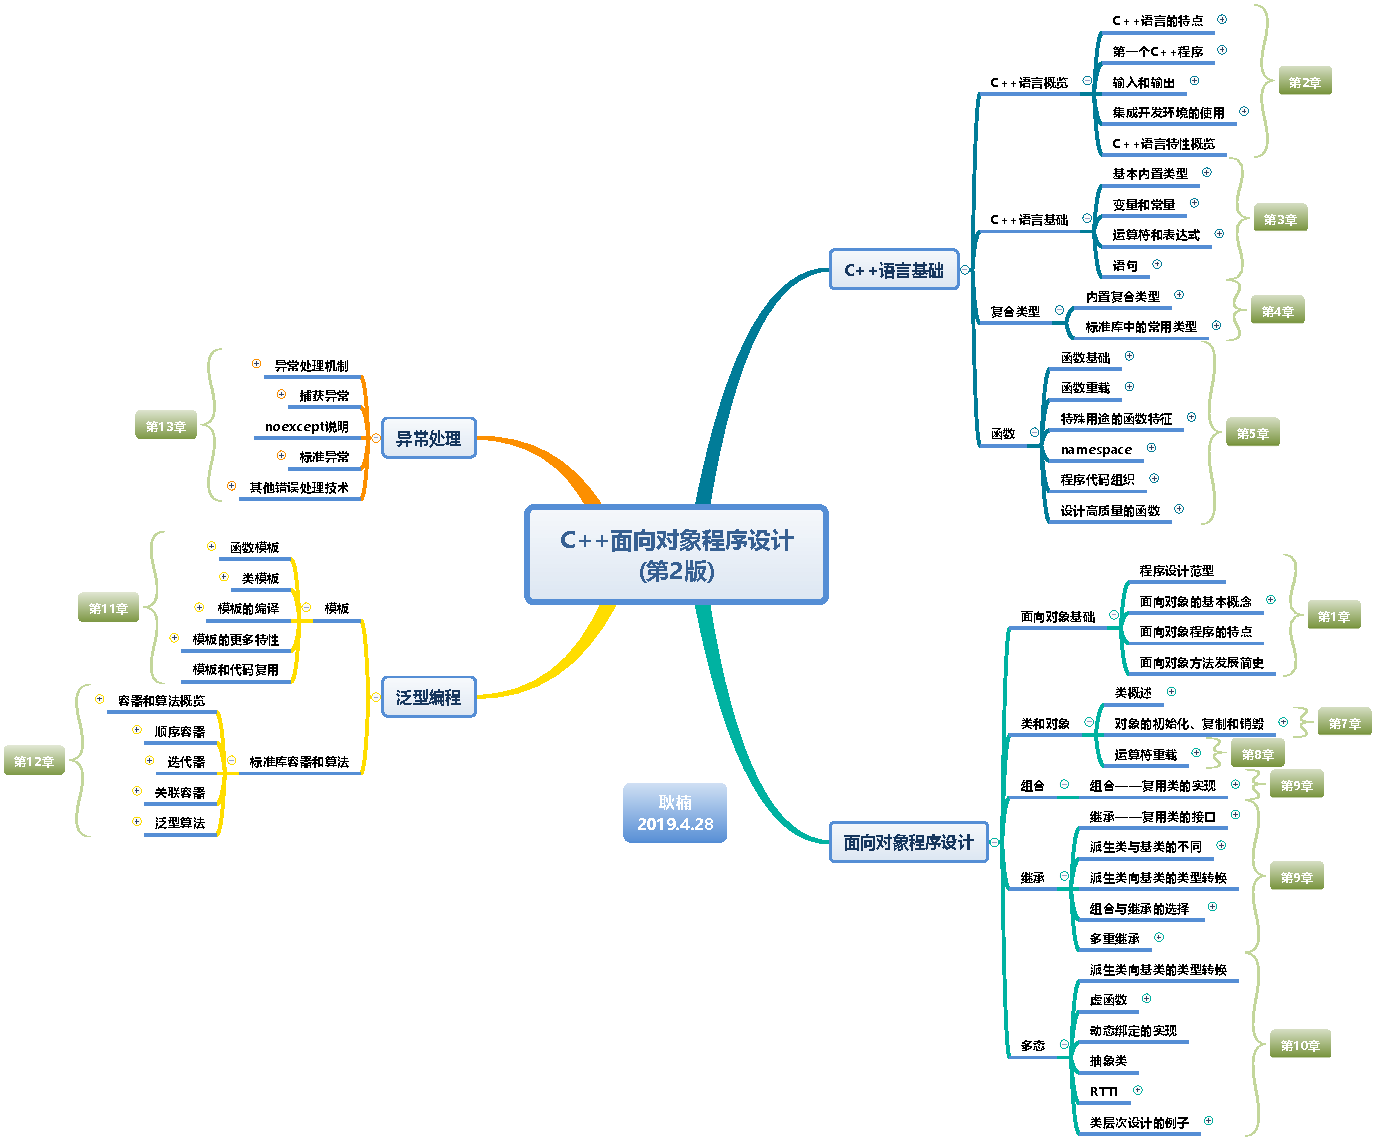
\includegraphics[height=0.8\textheight]{chap00/oopmindmap} %
  \stretchoff
\end{frame}

\begin{frame}{课程内容}{知识体系}
  \stretchon
  \begin{itemize}
  \item 学习路线
  \end{itemize}
  \centering
  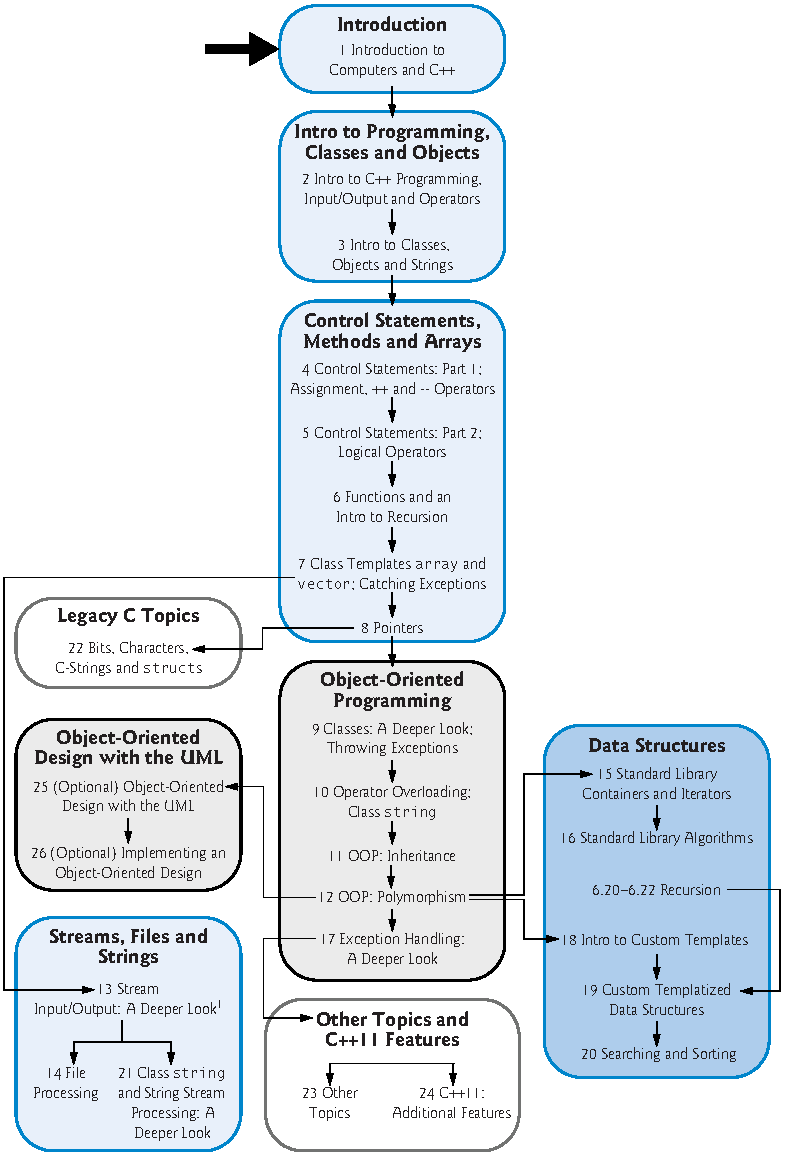
\includegraphics[height=0.8\textheight]{chap00/studyscheme} %
  \stretchoff
\end{frame}

%%%%%%%%%%%%%%%%%%%%%%%%%%%%%% 关于我 %%%%%%%%%%%%%%%%%%%%%%%%%%%%%%%%%%%
\section[关于我]{关于我}
\subsection[联系方式]{联系方式}
\begin{frame}[fragile]{关于我}{联系方式}
  % colour options
  \definecolor{seplinecolour}{HTML}{357f2d} % green
  \definecolor{iconcolour}{HTML}{2f3142} % dark
  \definecolor{textcolour}{HTML}{2f3142} % dark
  \definecolor{jobtitlecolour}{HTML}{474a65} % light dark

  % define some lengths for internal spacing
  \newlength{\seplinewidth} \setlength{\seplinewidth}{2cm}
  \newlength{\seplineheight} \setlength{\seplineheight}{1pt}
  \newlength{\seplinedistance} \setlength{\seplinedistance}{0.3cm}
  \begin{center}
    \begin{tikzpicture}
      % name
      \matrix[every node/.style={anchor=center,font=\huge},anchor=center] (name) {
        \node{耿\hspace{\ccwd}楠}; \\
        \node{\color{jobtitlecolour}\normalsize\textit{教授}}; \\
      };
      % sep line 1
      \node[below=0.3\seplinedistance of name] (hl1) {};
      \draw[line width=\seplineheight,color=seplinecolour] (hl1)++(-\seplinewidth/2,0) -- ++(\seplinewidth,0);
      % contact info
      \matrix [below=\seplinedistance of hl1,%
               column 1/.style={anchor=center,color=iconcolour},%
               column 2/.style={anchor=west}] (contact) {
        \node{\faGlobe}; & \node{\url{http://cie.nwsuaf.edu.cn/}};\\
        \node{\faBuilding}; & \node{信息工程学院};\\ 
        \node{\faEnvelope}; & \node{1234567890@nwafu.edu.cn};\\
        %\node{\faQq}; & \node{970291228};\\
        %\node{\faPhone}; & \node{15829540966}; \\
        \node{\faGithub}; & \node{\url{https://github.com/registor/}}; \\
      };
      %sep line 2
      \node[below=\seplinedistance of contact] (hl2) {};
      \draw[line width=\seplineheight,color=seplinecolour] (hl2)++(-\seplinewidth/2,0) -- ++(\seplinewidth,0);
      % interests
      \matrix [below=\seplinedistance of hl2,
         every node/.style={anchor=center,font=\LARGE}]
         (interests) {
        \node{\faCode}; & \node{\faCoffee}; &
        \node{\faLock}; & \node{\faWrench}; &
        \node{\faCameraRetro}; \\
      };
      
    \end{tikzpicture}
  \end{center}
\end{frame}
%%%%%%%%%%%%%%%%%%%%%%%%%%%%%%%%%%%%%%%%%%%%%%%%%%%%%%%%%%%%%%%%%%%%%%%%%%

%%% Local Variables: 
%%% mode: latex
%%% TeX-master: "../main.tex"
%%% End: 
